\documentclass[]{auvsi_doc}
\setkeys{auvsi_doc.cls}{
	AUVSITitle={Initial Concept Development}
	%AUVSILogoPath={./logo.pdf]}
}

% include extra packages, if needed
\usepackage{tikz, tikz-qtree}
\usepackage{longtable}


\begin{document}

\begin{AUVSITitlePage}
\begin{artifacttable}
\entry{CD-0001, 0.1, 2018-10-23, Initial Draft, John Akagi, [CHECKED BY]}
% additional \entry{} commands for extra rows in the revision table, if needed
\end{artifacttable}
\end{AUVSITitlePage}



\begin{longtable}[H]{|p{.15\columnwidth}|p{.34\columnwidth}|p{.12\columnwidth}|p{.34\columnwidth}|}
\hline
\textbf{Idea}	&	\textbf{Description}	&	\textbf{Decision} &	\textbf{Rationale} \\
\hline
Skycrane & UGV is lowered on a rope from the UAV & Investigate & Would eliminate the need for most cushioning and control surfaces on the UGV\\
\hline
Fins & Fins are used to give minimal control to a fast falling UGV & Investigate & Would be smaller than full glider wings but still allow decent control\\
\hline
Glider & Unpowered aircraft is used to control the falling UGV & Investigate & Would likely provide the greatest amount to control\\
\hline
Parasail & A controllable parachute is used to steer the UGV & Dropped & Difficult and unknown controls \\
\hline
Control Grids & Similar to SpaceX, grids are used to steer the descent of the UGV & Dropped & Too complex for this application \\
\hline
Magnus Effect & Spin the wheels of the UGV in the air to generate lift and control UGV attitude & Modify & Could be used in conjunction with other methods but unlikely to have much effect by itself\\
\hline
Autogyro & Unpowered helicopter rotors are used to slow descent and blades can be tilted to control the drop & Dropped & Mechanism was considered too complex \\
\hline
Bounce & UGV uses some elastic material under it to decrease the time of impact & Dropped & Bouncing would likely not reduce the impact forces to survivable levels \\
\hline
Airbag & An airbag is inflated just before lading to cushion the drop & Dropped & Needs precise measurements to determine when to inflate airbag, Airbag inflation mechanism is likely to require dangerous materials\\
\hline
Springs & Springs are placed under the UGV to absorb the energy from the drop & Modify & Could be used to reduce impact energy but unlikely to be able to dissipate all by itself \\
\hline
Counterweight & A large mass is ejected downwards just before impact in order to slow UGV descent & Dropped & Requires ejecting a large mass at high acceleration which is likely to be dangerous and impractical\\
\hline
Crumple Zone & Use a deformable material to break and absorb energy when UGV impacts ground & Modify & Could be used to reduce impact energy but unlikely to be able to dissipate all by itself\\
\hline
Balloons & Use balloons to increase drag and provide some lift & Dropped & Would be large and impractical to carry on board the UAV \\
\hline
Parachute & Use a parachute to slow the descent of the UGV & Investigate & Simplest idea and almost guaranteed to work \\
\hline
Seedpod & Attach a single propeller blade to the UGV which would cause the UGV to spin and slow its descent similar to how maple seeds work & Dropped & The UGV is likely too heavy to implement this properly\\
\hline
Nothing & Make the UGV as rugged as possible and drop it from the UAV with no slowing mechanism & Dropped & Any UGV that is rugged enough to survive a 100 ft drop would be too heavy and bulky to carry on the UAV \\
\hline
Low Drop & Drop below the minimum allowable flight level and drop the UGV from a lower altitude for increased survivability & Dropped & Would violate rules that state we must remain above a certain altitude\\
\hline

\caption{Description of initial ideas and decisions made. "Dropped" indicates the idea was considered unfeasible, "Investigate" indicates the idea was studied further, "Modify" indicates the idea was considered usable in conjunction with another idea or ideas. }
\end{longtable}



\begin{figure}
\centering
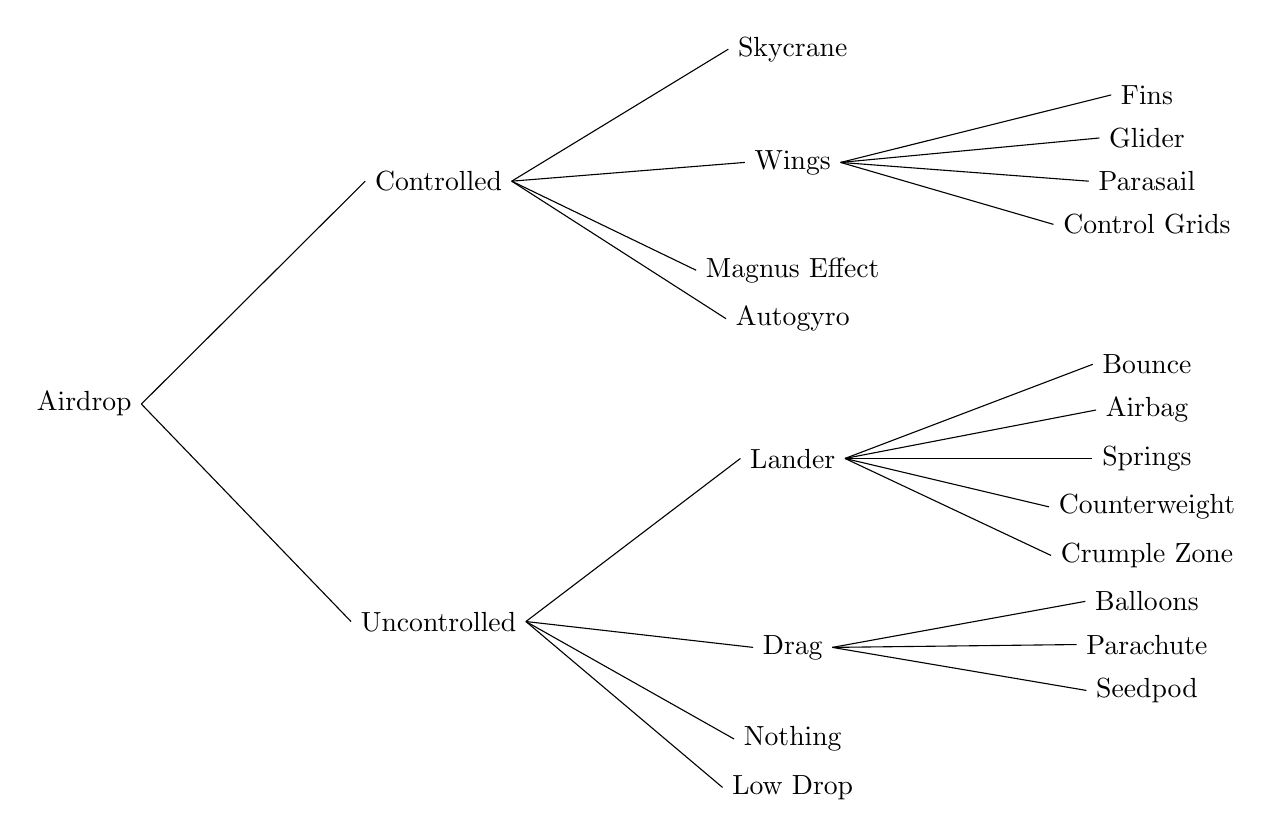
\begin{tikzpicture}
\tikzset{grow'=right,level distance=128pt}
\Tree[.Airdrop 	[.Controlled Skycrane [.Wings Fins Glider Parasail {Control Grids} ] {Magnus Effect} Autogyro ]
			[.Uncontrolled [.Lander Bounce Airbag Springs Counterweight {Crumple Zone} ] [.Drag Balloons Parachute Seedpod ] Nothing {Low Drop} ]]
\end{tikzpicture}
\caption{Concept development tree of the initial ideas generated for the payload delivery system.}
\label{fig:ConceptTree}
\end{figure}



\end{document}